\usetikzlibrary{arrows,shapes,chains}
\section{任务规划}
\frame
{
  \frametitle{\secname~ }
  \begin{columns}[onlytextwidth]
  \begin{column}{0.35\textwidth}
  \begin{block}{计划}
  \begin{itemize}
    \item 论文写作
    \item 学习《机器学习》
    \item 学习英语
  \end{itemize}
  \end{block}
  \end{column}
  \hspace{0.5em}
  \begin{column}{0.65\textwidth}
    \begin{block}{实际}
      \begin{itemize}
        \item 完成初稿,熟练使用latex
        \item 学习了4章
        \item 完成一篇专利的初稿
      \end{itemize}
    \end{block}
  \end{column}
  \end{columns}
  \note{
    笔记
  }
}

\subsection{论文写作}
\frame{
  \frametitle{论文写作}
  \begin{figure}  
  \tikzstyle{format}=[rectangle,draw,thin,fill=white]  
  %定义语句块的颜色,形状和边
  \tikzstyle{test}=[diamond,aspect=2,draw,thin]  
  %定义条件块的形状,颜色
  \tikzstyle{point}=[coordinate,on grid,]  
  %像素点,用于连接转移线
  \begin{tikzpicture}
    %[node distance=10mm,auto,>=latex',thin,start chain=going below,every join/.style={norm},] 
  %start chain=going below指明了流程图的默认方向,node distance=8mm则指明了默认的node距离。这些可以在定义node的时候更改,比如说 
  %\node[point,right of=n3,node distance=10mm] (p0){};  
  %这里声明了node p0,它在node n3 的右边,距离是10mm。
  	%\node[format] (n0) at(4,4){A}; 直接指定位置 
		%定义完node之后进行连线,
		%\draw[->] (n0.south) -- (n1); 带箭头实线
		%\draw[-] (n0.south) -- (n1); 不带箭头实线
		%\draw[<->] (n0.south) -- (n1.north);   双箭头
		%\draw[<-,dashed] (n1.south) -- (n2.north); 带箭头虚线 
		%\draw[<-] (n0.south) to node{Yes} (n1.north);  带字,字在箭头方向右边
		%\draw[->] (n1.north) to node{Yes} (n0.south);  带字,字在箭头方向左边
		%\draw[->] (n1.north) to[out=60,in=300] node{Yes} (n0.south);  曲线
		%\draw[->,draw=red](n2)--(n1);  带颜色的线
  \node[format] (start){阅读论文};
  \node[format,below of=start,node distance=10mm] (define){查阅相关文献};
  \node[format,below of=define,node distance=10mm] (PCFinit){复现文献};
  \node[format,below of=PCFinit,node distance=10mm] (DS18init){完成中文初稿};
  \node[format,below of=DS18init,node distance=10mm] (LCDinit){修改并翻译中文草稿};
  \node[format,below of=LCDinit,node distance=10mm] (processtime){修改英文论文};
  \draw[->] (start)--(define);
  \draw[->] (define)--(PCFinit);
  \draw[->](PCFinit)--(DS18init);
  \draw[->](DS18init)--(LCDinit);
  \draw[->](LCDinit)--(processtime);
\end{tikzpicture}  
\end{figure} 
%%%%%%%%%%%%%%%%%%----------批量插入图片------------%%%%%%%%%%%%%
  % \begin{figure}
  %   \hspace{-2.0em}
  %   \begin{minipage}{1.06\textwidth}
  %     \subfloat[\scriptsize AABB]
  %     {
  %       \includegraphics[width=0.2\textwidth]{figures/bunny-2d-AABB.eps}
  %     }
  %     \subfloat[\scriptsize OBB]
  %     {
  %       \includegraphics[width=0.2\textwidth]{figures/bunny-2d-OBB.eps}
  %     }
  %     \subfloat[\scriptsize Sphere]
  %     {
  %       \includegraphics[width=0.2\textwidth]{figures/bunny-2d-Sphere.eps}
  %     }%\linebreak
  %     \subfloat[\scriptsize $k$-DOP]
  %     {
  %       \includegraphics[width=0.2\textwidth]{figures/bunny-2d-8DOP.eps}
  %     }
  %     \subfloat[\scriptsize 凸包]
  %     {
  %       \includegraphics[width=0.2\textwidth]{figures/bunny-2d-Convexhull.eps}
  %     }
  %   \end{minipage}
  %   \caption{不同种类的包围体}
  %   \label{chart:exps:tightness}
  % \end{figure}
  % \vspace{-1em}
  % 其他:Tribox、Swept-sphere、 Sphere-shell、Zonotopes、圆柱形、圆锥、椭球形等等。

  \note{
    上面这几个就是最常见的凸包围体。最常见的沿坐标轴方向的AABB包围盒,带方向的包围盒OBB,包围球,k面的凸包围体(k-DOP),和凸包,还有一些比较特定领域用的圆柱、圆锥形、椭球形等等。
    其中k-DOP是采用k/2对固定方向的半空间相交构成的凸包围体,是综合比较较好的包围体,因为可以通过k来调节包围体的简单性和紧致性来满足不同应用的需求。
  }
}

\frame{
  \frametitle{学习《机器学习》}
  \footnotesize
  %\textbf  加粗
  计划啃完整本,最后看了\textbf{决策树}、\textbf{神经网络}、\textbf{支持向量机}、\textbf{贝叶斯分类器}、\\
  \textbf{集成学习}、\textbf{聚类}、\textbf{概率图模型}
  \begin{block}{收获}
    \hspace{-2.0em}   \begin{minipage}{\textwidth}
      \begin{description}
        \item[机器学习] 了解并推导常见机器学习算法
        \item[概率图模型] 学习概率图模型的推理,参数学习算法\\
                        在王昊的指导下,学习Soble指数法
        \item[基础知识] 有了理论基础,发现以前的很多表述不够准确
      \end{description}
    \end{minipage}
  \end{block}

  \note{
    描述PPT。

  }
}

\subsection{latex绘制贝叶斯网络}
\frame{
  \frametitle{\subsecname~ }
  \begin{figure}[!]
    \begin{minipage}[c]{5cm}  
    \resizebox{!}{3cm}{%
    \parbox{4cm}{
\usetikzlibrary{positioning,arrows.meta,quotes}
\usetikzlibrary{shapes,snakes}
\usetikzlibrary{bayesnet}
\tikzset{>=latex}
\tikzstyle{plate caption} = [caption, node distance=0, inner sep=0pt,
below left=5pt and 0pt of #1.south]
 

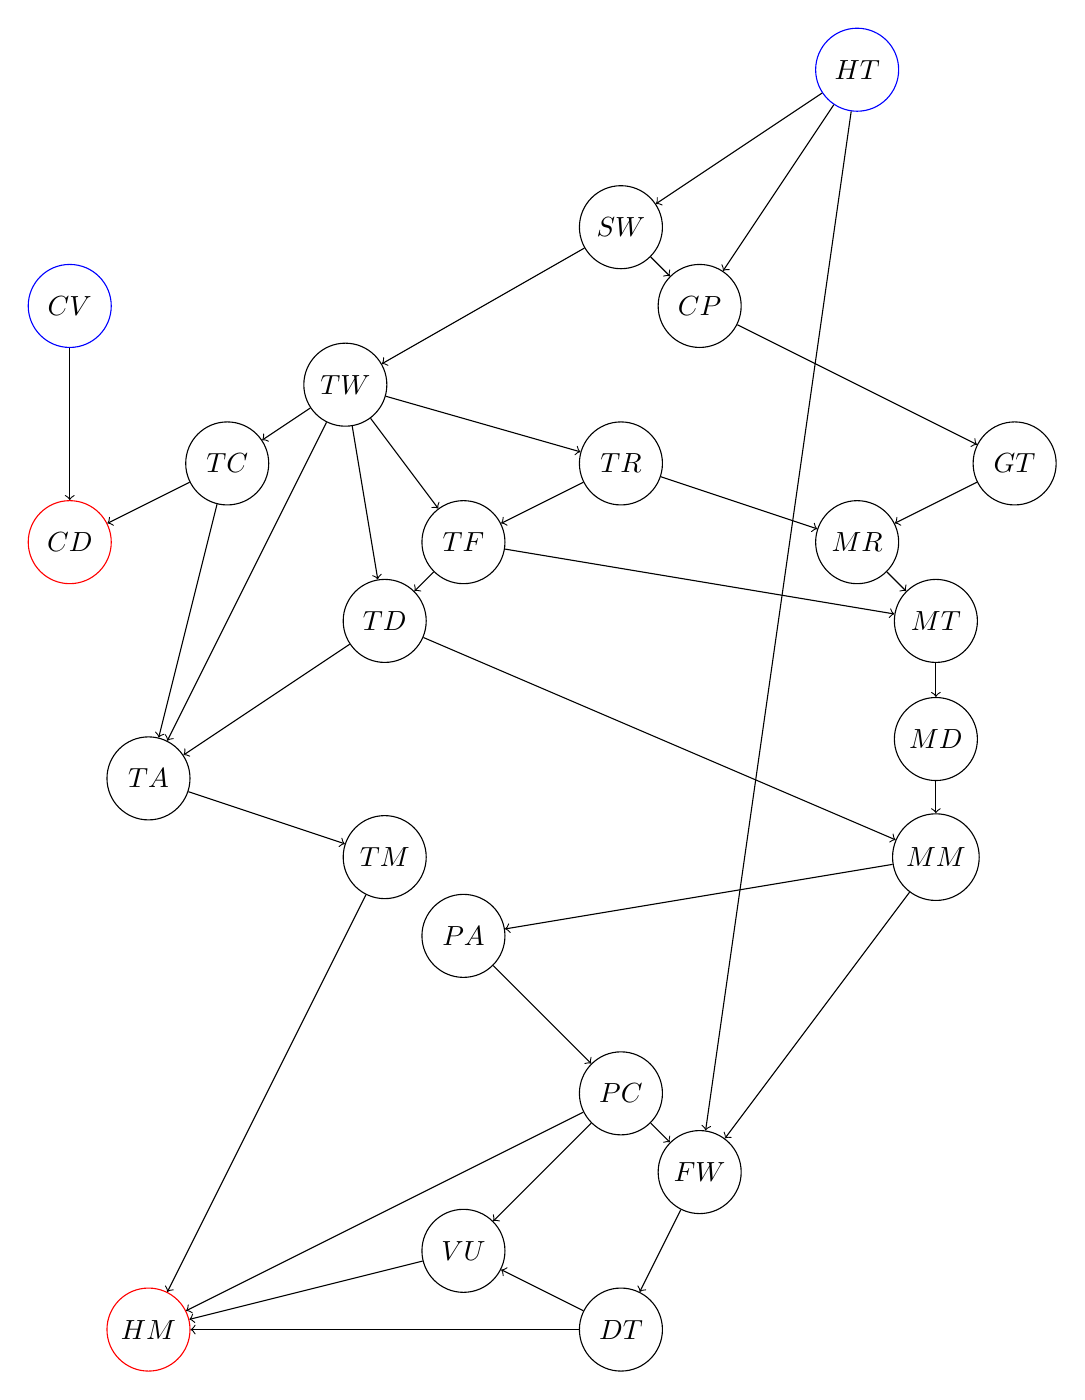
\begin{tikzpicture}
%     \begin{comment}
%     \node[circle,minimum width =30pt ,minimum height =30pt ,draw=blue] (1) at(4,16){$CV$};
% \node[circle,minimum width =30pt ,minimum height =30pt ,draw=blue] (2) at(14,19){$HT$};
% \node[circle,minimum width =30pt ,minimum height =30pt ,draw=blue] (3) at(11,17){$SW$};
% \node[circle,minimum width =30pt ,minimum height =30pt ,draw=blue] (4) at(7.5,15){$TW$};
% \node[circle,minimum width =30pt ,minimum height =30pt ,draw=blue] (5) at(6,14){$TC$};
% \node[circle,minimum width =30pt ,minimum height =30pt ,draw=blue] (6) at(4,13){$CD$};
% \node[circle,minimum width =30pt ,minimum height =30pt ,draw=blue] (7) at(11,14){$TR$};
% \node[circle,minimum width =30pt ,minimum height =30pt ,draw=blue] (8) at(9,13){$TF$};
% \node[circle,minimum width =30pt ,minimum height =30pt ,draw=blue] (9) at(8,12){$TD$};
% \node[circle,minimum width =30pt ,minimum height =30pt ,draw=blue] (10) at(5,10){$TA $};
% \node[circle,minimum width =30pt ,minimum height =30pt ,draw=blue] (11) at(8,9){$TM$};
% \node[circle,minimum width =30pt ,minimum height =30pt ,draw=blue] (12) at(12,16){$CP$};
% \node[circle,minimum width =30pt ,minimum height =30pt ,draw=blue] (13) at(16,14){$GT$};
% \node[circle,minimum width =30pt ,minimum height =30pt ,draw=blue] (14) at(14,13){$MR$};
% \node[circle,minimum width =30pt ,minimum height =30pt ,draw=blue] (15) at(15,12){$MT$};
% \node[circle,minimum width =30pt ,minimum height =30pt ,draw=blue] (16) at(15,10.5){$MD$};
% \node[circle,minimum width =30pt ,minimum height =30pt ,draw=blue] (17) at(15,9){$MM $};
% \node[circle,minimum width =30pt ,minimum height =30pt ,draw=blue] (18) at(9,8){$PA$};
% \node[circle,minimum width =30pt ,minimum height =30pt ,draw=blue] (19) at(11,6){$PC$};
% \node[circle,minimum width =30pt ,minimum height =30pt ,draw=blue] (20) at(12,5){$FW$};
% \node[circle,minimum width =30pt ,minimum height =30pt ,draw=blue] (21) at(11,3){$DT$};
% \node[circle,minimum width =30pt ,minimum height =30pt ,draw=blue] (22) at(9,4){$VU$};
% \node[circle,minimum width =30pt ,minimum height =30pt ,draw=blue] (23) at(5,3){$HM$};
%     \end{comment}

\node[circle,minimum width =30pt ,minimum height =30pt ,draw=blue] (1) at(4,16){$CV$};
\node[circle,minimum width =30pt ,minimum height =30pt ,draw=blue] (2) at(14,19){$HT$};
\node[circle,minimum width =30pt ,minimum height =30pt ,draw=black] (3) at(11,17){$SW$};
\node[circle,minimum width =30pt ,minimum height =30pt ,draw=black] (4) at(7.5,15){$TW$};
\node[circle,minimum width =30pt ,minimum height =30pt ,draw=black] (5) at(6,14){$TC$};
\node[circle,minimum width =30pt ,minimum height =30pt ,draw=red] (6) at(4,13){$CD$};
\node[circle,minimum width =30pt ,minimum height =30pt ,draw=black] (7) at(11,14){$TR$};
\node[circle,minimum width =30pt ,minimum height =30pt ,draw=black] (8) at(9,13){$TF$};
\node[circle,minimum width =30pt ,minimum height =30pt ,draw=black] (9) at(8,12){$TD$};
\node[circle,minimum width =30pt ,minimum height =30pt ,draw=black] (10) at(5,10){$TA $};
\node[circle,minimum width =30pt ,minimum height =30pt ,draw=black] (11) at(8,9){$TM$};
\node[circle,minimum width =30pt ,minimum height =30pt ,draw=black] (12) at(12,16){$CP$};
\node[circle,minimum width =30pt ,minimum height =30pt ,draw=black] (13) at(16,14){$GT$};
\node[circle,minimum width =30pt ,minimum height =30pt ,draw=black] (14) at(14,13){$MR$};
\node[circle,minimum width =30pt ,minimum height =30pt ,draw=black] (15) at(15,12){$MT$};
\node[circle,minimum width =30pt ,minimum height =30pt ,draw=black] (16) at(15,10.5){$MD$};
\node[circle,minimum width =30pt ,minimum height =30pt ,draw=black] (17) at(15,9){$MM $};
\node[circle,minimum width =30pt ,minimum height =30pt ,draw=black] (18) at(9,8){$PA$};
\node[circle,minimum width =30pt ,minimum height =30pt ,draw=black] (19) at(11,6){$PC$};
\node[circle,minimum width =30pt ,minimum height =30pt ,draw=black] (20) at(12,5){$FW$};
\node[circle,minimum width =30pt ,minimum height =30pt ,draw=black] (21) at(11,3){$DT$};
\node[circle,minimum width =30pt ,minimum height =30pt ,draw=black] (22) at(9,4){$VU$};
\node[circle,minimum width =30pt ,minimum height =30pt ,draw=red] (23) at(5,3){$HM$};

    \draw[->] (1) --(6);
\draw[->] (2) --(3);
\draw[->] (2) --(12);
\draw[->] (2) --(20);
\draw[->] (3) --(4);
\draw[->] (3) --(12);
\draw[->] (4) --(5);
\draw[->] (4) --(7);
\draw[->] (4) --(8);
\draw[->] (4) --(9);
\draw[->] (4) --(10);
\draw[->] (5) --(6);
\draw[->] (5) --(10);
\draw[->] (7) --(8);
\draw[->] (7) --(14);
\draw[->] (8) --(9);
\draw[->] (8) --(15);
\draw[->] (9) --(10);
\draw[->] (9) --(17);
\draw[->] (10) --(11);
\draw[->] (11) --(23);
\draw[->] (12) --(13);
\draw[->] (13) --(14);
\draw[->] (14) --(15);
\draw[->] (15) --(16);
\draw[->] (16) --(17);
\draw[->] (17) --(18);
\draw[->] (17) --(20);
\draw[->] (18) --(19);
\draw[->] (19) --(20);
\draw[->] (19) --(22);
\draw[->] (19) --(23);
\draw[->] (20) --(21);
\draw[->] (21) --(22);
\draw[->] (21) --(23);
\draw[->] (22) --(23);


\end{tikzpicture}

}
    }
    \end{minipage}
  \end{figure}


  \note{
    (介绍PPT后)
  }
}

% \frame{
%   \frametitle{基于~BVH~的碰撞检测算法}
%   \begin{columns}[onlytextwidth]
%     \begin{column}{0.35\textwidth}
%       \vspace{-1.5em}
%       \begin{figure}[htbp]
%         \begin{center}
%           \begin{boxedminipage}{1\textwidth}
%             \subfloat{\label{lbl:bvh-bunny-center-0.png}}
%             {\includegraphics[height=1.4cm]{bvh-bunny-center-0.png}}
%             \subfloat{\label{lbl:bvh-bunny-center-1.png}}
%             {\includegraphics[height=1.4cm]{bvh-bunny-center-1.png}}
%             \\
%             \subfloat{\label{lbl:bvh-bunny-center-2.png}}
%             {\includegraphics[height=1.4cm]{bvh-bunny-center-2.png}}
%             \subfloat{\label{lbl:bvh-bunny-center-3.png}}
%             {\includegraphics[height=1.4cm]{bvh-bunny-center-3.png}}
%             \\\hspace{0.5cm}
%             \subfloat{\label{lbl:bvh-bunny-center-4.png}}
%             {\includegraphics[height=1.5cm]{bvh-bunny-center-4.png}}
%             \subfloat{\label{lbl:bvh-bunny-center-5.png}}
%             {\includegraphics[height=1.5cm]{bvh-bunny-center-5.png}}
%             \\
%             \subfloat{\label{lbl:bvh-bunny-center-6.png}}
%             {\includegraphics[height=1.5cm]{bvh-bunny-center-6.png}}
%             \subfloat{\label{lbl:bvh-bunny-center-7.png}}
%             {\includegraphics[height=1.5cm]{bvh-bunny-center-7.png}}
%           \end{boxedminipage}
%           \vspace{-0.5em}
%           \caption{八层~BVH~示例}
%           \label{lbl:bvh-example}
%         \end{center}
%       \end{figure}
%     \end{column}
%     \hspace{0.5em}
%     \begin{column}{1.2\textwidth}
%       \vspace{0.2em}
%       \scalebox{0.5}{
%         \begin{minipage}{1.0\textwidth}
%           \vspace{-2em}
%           \begin{algorithm}[H]
%             \caption{自顶向下层次遍历~BVH~}
%             \label{alg:traverse-bvh-tree}
%             \begin{algorithmic}[1]
%               \Require
%               两个~BVH~树的根节点~$node_1$,$node_2$
%               \Ensure
%               模型是否相交
%               \Function {TraverseBVHTree}{$node_1, node_2$}
%               \If{$node_1.bv \cap node_2.bv = \emptyset$}
%               \State \Return{\textbf{False}}
%               \Comment{包围体重合测试, 包围体不相交直接返回}
%               \Else
%               \If {$node_1.children = \emptyset$}
%               \If {$node_2.children = \emptyset$}
%               \State \Comment{最底层叶子节点原生几何相交测试}
%               \State \Return {\Call{CheckIntersection}{$node_1.primitives, node_2.primitives$}}
%               \Else
%               \ForAll {$child \in node_2.children$}
%               \State \Call{TraverseBVHTree}{$node_1, child$} \Comment{递归调用}
%               \EndFor
%               \EndIf
%               \Else
%               \ForAll {$child \in node_1.children$}
%               \State \Call{TraverseBVHTree}{$child, node_2$}  \Comment{递归调用}
%               \EndFor
%               \EndIf
%               \EndIf
%               \EndFunction
%             \end{algorithmic}
%           \end{algorithm}
%         \end{minipage}
%       }
%       \\
%       \scriptsize \hspace{1em}代价函数: $T_{cost} = n_v * C_v + n_p * C_p + (n_u * C_u)$(运动)
%     \end{column}
%   \end{columns}
%   \note{
%     基于包围体树的碰撞检测算法, 一般首先都会初始化环境然后构建层次结构的包围体树,碰撞检测时从顶层开始逐渐往下层遍历,到最底层叶子节点后开始三角网格模型相交测试,
%     当发现三角网格相交后立即终止遍历,确定模型发生碰撞。
%     评价碰撞检测算法的指标一般用上面这个公式来衡量,其中nv和 np分别表示参与包围体节点相交测试的数量和参与原始几何相交测试的数量,Cv和 Cp则表示相应的平均测试耗费的代价。
%     当在运动场景时还需要加上nu和 Cn就是模型旋转或者运动后包围体更新的数量和更新的代价。
%     本文算法就是尽早发现包围体不相交的情况,减少np和cp的数量。
%   }
% }
